\label{sec:mute-topologie-protocole-diffusion}

Netflux établit un réseau \ac{P2P} par document.
Chacun de ces réseaux est un réseau entièrement maillé : chaque noeud se connecte à l'ensemble des autres noeuds.
Nous illustrons cette topologie par la \autoref{fig:full-meshed-topology}.

\begin{figure}[!ht]
    \centering
    \resizebox{0.5 \columnwidth}{!}{
        \begin{tikzpicture}
            \path
                +(90:10) node (a) {\includegraphics[page=5, trim=0cm 24cm 32cm 0cm, clip]{img/mute-figures.pdf}}
                +(-90:10) node (b) {\includegraphics[page=5, trim=0cm 24cm 32cm 0cm, clip]{img/mute-figures.pdf}}
                +(180:5) node (c) {\includegraphics[page=5, trim=0cm 24cm 32cm 0cm, clip]{img/mute-figures.pdf}}
                ++(0:10)
                +(90:10) node (d) {\includegraphics[page=5, trim=0cm 24cm 32cm 0cm, clip]{img/mute-figures.pdf}}
                +(-90:10) node (e) {\includegraphics[page=5, trim=0cm 24cm 32cm 0cm, clip]{img/mute-figures.pdf}}
                +(0:5) node (f) {\includegraphics[page=5, trim=0cm 24cm 32cm 0cm, clip]{img/mute-figures.pdf}};

            \draw[latex-latex, line width=1.5mm]
                (a) edge (b) (a) edge (c) (a) edge (d) (a) edge (e) (a) edge (f)
                (b) edge (c) (b) edge (d) (b) edge (e) (b) edge (f)
                (c) edge (d) (c) edge (e) (c) edge (f)
                (d) edge (e) (d) edge (f)
                (e) edge (f);
        \end{tikzpicture}
    }
    \caption{Topologie réseau entièrement maillée}
    \label{fig:full-meshed-topology}
  \end{figure}

Cette topologie présente les avantages suivants :
\begin{enumerate}
    \item Sa simplicité.
    \item Le nombre de sauts entre les noeuds, minimal, qui permet de minimiser le délai de communication.
    \item La redondance de ses routes, qui permet aux noeuds de continuer à communiquer même en cas de défaillance d'une ou plusieurs routes.
\end{enumerate}

Cependant, cette topologie est limitée par sa capacité de passage à l'échelle.
En effet, elle implique un nombre de connexions qui dépend linéairement du nombre de noeuds.
Chacune de ces connexions impliquant un coût, cette topologie n'est adaptée qu'à des groupes de taille réduite.

De plus, nous associons à cette topologie réseau un protocole de diffusion des messages tout aussi simple : lorsqu'un noeud effectue une modification, il diffuse le message correspondant à l'ensemble des noeuds, \ie il envoie une copie du message à chacun des noeuds.
La charge de travail pour la diffusion d'un message est donc assumée uniquement par son auteur, ce qui s'avère prohibitif dans le cadre de collaborations à large échelle. \\

Afin de supporter des collaborations à large échelle, il est donc nécessaire de mettre en place :
\begin{enumerate}
    \item Une topologie limitant le nombre de connexions par noeud.
    \item Un protocole de diffusion des messages répartissant la charge entre les noeuds.
\end{enumerate}

Le protocole d'échantillonnage aléatoire de pairs adaptatif Spray \cite{2018-spray-nedelec} répond à notre première limite.
Ce protocole permet d'établir un réseau \ac{P2P} connecté.
Toutefois, la topologie adoptée limite le voisinage de chaque noeud, \ie le nombre de connexions que chaque noeud possède, à un facteur logarithmique par rapport au nombre total de noeuds.
De plus, ce protocole est adapté à un réseau \ac{P2P} dynamique, \ie il ajuste le voisinage des noeuds au fur et à mesure des connexions et déconnexions des noeuds.

La topologie résultante est propice à l'emploi d'un protocole de diffusion épidémique des messages, tel que celui utilisé par SWIM \cf{sec:swim-update-dissemination}.
Pour rappel, ce type de protocole consiste à ce qu'un noeud ne diffuse un message qu'à un sous-ensemble de ses voisins.
À la réception de son message, ses voisins diffusent à leur tour le message à une partie de leur voisinage, et ainsi de suite.
L'emploi de ce type de protocole permet ainsi de répartir entre les noeuds la charge de travail nécessaire à la diffusion du message à l'ensemble des noeuds.

Ces modifications rendraient donc viables les collaborations à large échelle sur \ac{MUTE}.
En contrepartie, le délai nécessaire pour la diffusion d'une modification augmenterait, \ie le temps nécessaire pour qu'une modification effectuée par un noeud soit intégrée par les autres noeuds.
Il s'agit toutefois d'un compromis que nous jugeons nécessaire.
